\chapter{rogettazione logica}
\section{Stima del volume dei dati}
\begin{table}[H]
  \centering
  \rowcolors{2}{green!80!black!40}{white}
  \begin{tabular}{|c|c|c|}
    \hline
    \rowcolor{green!70!black!80}
    \textbf{Concetto} & \textbf{Costrutto} & \textbf{Volume} \\
    \hline
    Centri & E & 84 \\
    Posizioni & E & 166 \\
    Settori & E & 125 \\
    Controllori & E & 4200 \\
    Ferie & E & 8400 \\
    Abilitazione & E & 4200 \\
    Turni (mensili) & E & 20000 \\
    Aerodromi & E & 43 \\
    Piste & E & 43 \\
    Punti & E & 3750 \\
    Piani di volo (mensili) & E & 5000 \\
    Aereomobili & E & 5000 \\
    Composizione (settori postazioni) & R & 125 \\
    Abilitamento (abilitazioni settori) & R & 4200 \\
    Stimati & R & 500.000 \\
    Percorrenza & R & 500.000 \\
    \hline
  \end{tabular}
  \end{table}
  \section{Descrizione delle operazioni principali e stima della loro frequenza}

  \begin{table}[H]
  \centering
  \rowcolors{2}{green!80!black!40}{white}
  \begin{tabular}{|c|c|c|}
  \hline
  \rowcolor{green!70!black!80}
  \textbf{Codice} & \textbf{Operazione} & \textbf{Frequenza stimata} \\
  \hline
  OP1 & Aggiunta e/o rimozione di un nuovo controllore di volo & 3 al mese \\
  OP2 & Modifica dei dati personali di un controllore di volo & 10 al mese \\
  OP3 & Assegnazione delle ferie a un controllore di volo & 100 al mese \\
  OP4 & Aggiunta di un'abilitazione a un controllore di volo & 50 al mese \\
  OP5 & Calcolo dei turni mensili per i controllori di volo & 1 al mese \\
  OP6 & Aggiunta di un nuovo piano di volo & 2000 al mese \\
  OP7 & Rimozione di un piano di volo & 100 al mese \\
  OP8 & Modifica di un piano di volo esistente & 1500 al mese \\
  OP9 & Aggiunta e/o rimozione di un nuovo aereomobile & 50 al mese \\
  OP10 & Calcolo del ral & 1 all'anno \\
  OP11 & Stima dei voli in un settore in un ora & 500.000 al mese \\
  OP12 & Aggiunta di una percorrenza & 500.000 al mese \\

  \hline
  \end{tabular}
  \end{table}
  
  La tabella sopra riportata fornisce un elenco delle operazioni principali che possono essere eseguite nel sistema di gestione del personale di controllo del traffico aereo. Per ciascuna operazione, viene fornita una stima numerica della loro frequenza stimata al mese.
\section{Schemi di navigazione e tabelle degli accessi}
Sono riportate in seguito le tabelle degli accessi delle operazioni sopra riportate, inoltre, ove
non risulti banale, sono stati inseriti i relativi schemi di navigazione. Al fine del calcolo degli
costi, si considerano di peso doppio gli accessi in scrittura rispetto a quelli in lettura.

\subsection*{OP1 - Modifica dei dati personali di un controllore di volo}
\begin{table}[H]
  \centering
  \rowcolors{2}{green!80!black!40}{white}
  \begin{tabular}{|c|c|c|c|}
  \hline
  \rowcolor{green!70!black!80}
  \textbf{Concetto} & \textbf{Costrutto} & \textbf{accessi} & \textbf{tipo}\\
  \hline
  Controllore & E & 1 & S \\
  &  & Totale: 1S, 6 al mese &\\
  \hline
  \end{tabular}
  \end{table}

    \subsection*{OP2 - Modifica dei dati personali di un controllore di volo}
    \begin{table}[H]
      \centering
      \rowcolors{2}{green!80!black!40}{white}
      \begin{tabular}{|c|c|c|c|}
      \hline
      \rowcolor{green!70!black!80}
      \textbf{Concetto} & \textbf{Costrutto} & \textbf{accessi} & \textbf{tipo}\\
      \hline
      Controllore & E & 1 & L \\
      Controllore & E & 1 & S \\
      &  & Totale: 1S 1L, 30 al mese &\\
      \hline
      \end{tabular}
      \end{table}
  
      \subsection*{OP3 - Assegnazione delle ferie a un controllore di volo}
      \begin{table}[H]
    \centering
    \rowcolors{2}{green!80!black!40}{white}
    \begin{tabular}{|c|c|c|c|}
    \hline
    \rowcolor{green!70!black!80}
    \textbf{Concetto} & \textbf{Costrutto} & \textbf{accessi} & \textbf{tipo}\\
    \hline
    Controllore & E & 1 & L \\
    Ferie & E & 1 & S \\
    & & Totale: 1S, 1L, 300 al mese &\\
    \hline
    \end{tabular}
    \end{table}

    \subsection*{OP4 - Aggiunta di un'abilitazione a un controllore di volo}
    \begin{table}[H]
    \centering
    \rowcolors{2}{green!80!black!40}{white}
    \begin{tabular}{|c|c|c|c|}
    \hline
    \rowcolor{green!70!black!80}
    \textbf{Concetto} & \textbf{Costrutto} & \textbf{accessi} & \textbf{tipo}\\
    \hline
    Controllore & E & 1 & L \\
    Abilitamento & R & 1 & S \\
    Abilitazione & E & 1 & S \\
    & & Totale: 2S, 1L, 250 al mese &\\
    \hline
    \end{tabular}
    \end{table}

    \subsection*{OP5 - Calcolo dei turni mensili per i controllori di volo}
    \begin{table}[H]
    \centering
    \rowcolors{2}{green!80!black!40}{white}
    \begin{tabular}{|c|c|c|c|}
    \hline
    \rowcolor{green!70!black!80}
    \textbf{Concetto} & \textbf{Costrutto} & \textbf{accessi} & \textbf{tipo}\\
    \hline
    Controllore & E & 4200 & L \\
    Turno & E & 20000 & L \\
    Stimato & E & 500.000 & L \\
    Postazione & E & 166 & L \\
    Settore & E & 125 & L \\
    & & Totale: 0S, 524,491L, 524.491 al mese &\\
    \hline
    \end{tabular}
    \end{table}
    Per ogni turno e per ogni posizione viene calcolata l'occupazione e viene cercato il controllore adatto con meno turni lavorati.
    Il modo con cui conteggiamo le letture non tiene conto delle ricerce, l'operazine effettiva sul calcolatore è estremamente pesante.
    \begin{figure}[H]
      \centering
      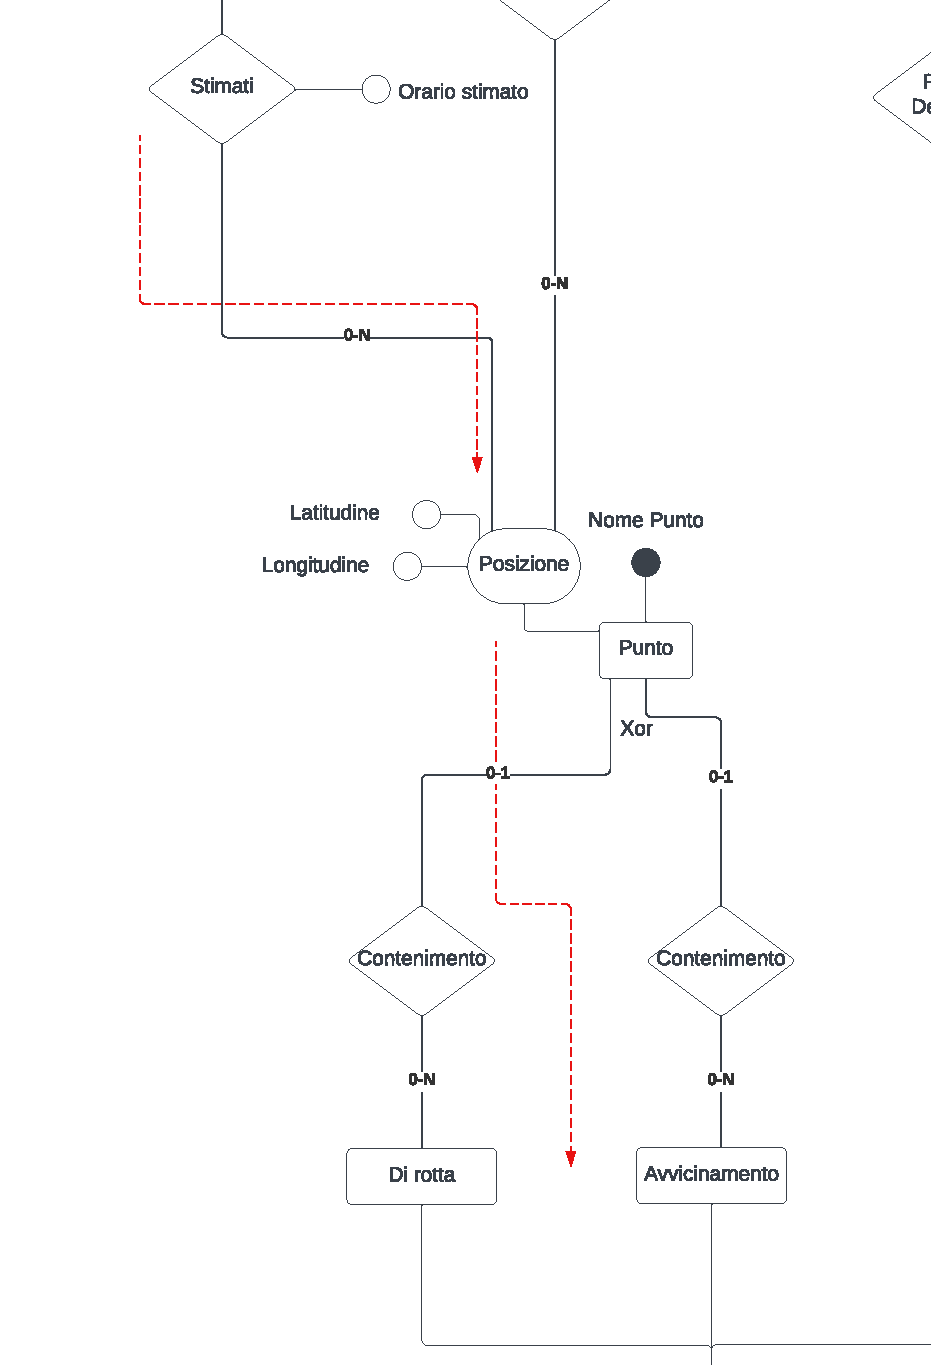
\includegraphics[width=10cm]{figures/BasicControllerarrowsp1.pdf}
      \caption{"Percorso per trovare l'occupazione"}
    \end{figure}
    \begin{figure}[H]
      \centering
      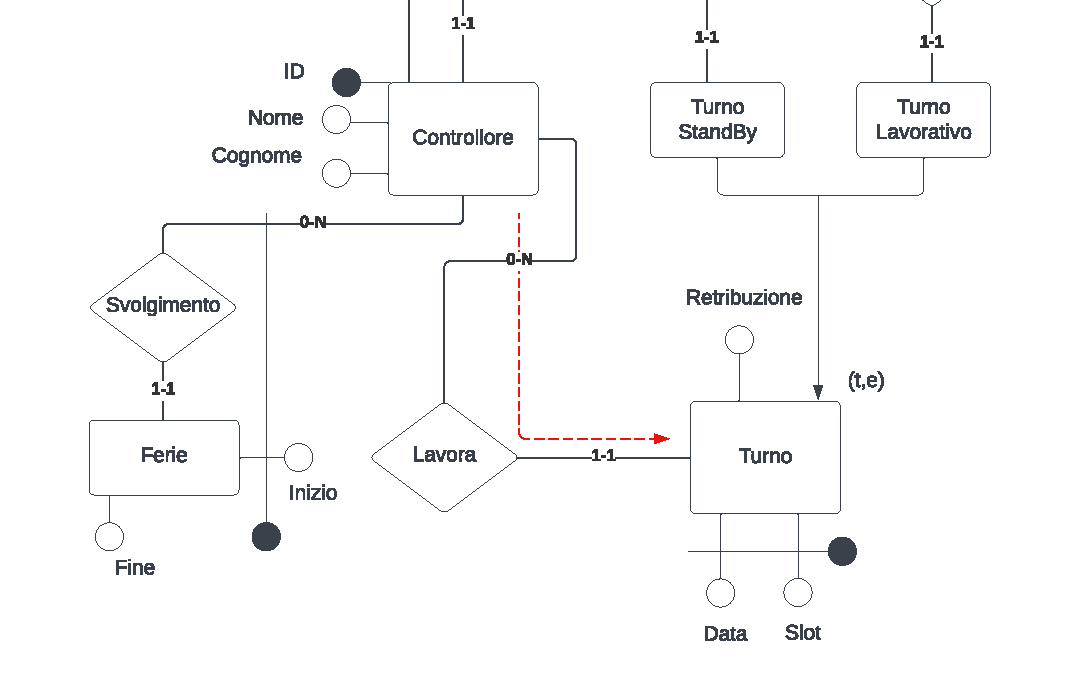
\includegraphics[width=1\textwidth]{figures/BasicControllerarrowsp2.pdf}
      \caption{"Percorso per trovare I turni lavorati"}
    \end{figure}

    \subsection*{OP6 - Aggiunta di un nuovo piano di volo}
    \begin{table}[H]
    \centering
    \rowcolors{2}{green!80!black!40}{white}
    \begin{tabular}{|c|c|c|c|}
    \hline
    \rowcolor{green!70!black!80}
    \textbf{Concetto} & \textbf{Costrutto} & \textbf{accessi} & \textbf{tipo}\\
    \hline
    Piano di Volo & E & 1 & S \\
    Stimati & E & 100 & S \\
    Punti & E & 100 & R \\
    Piste & E & 2 & R \\
    Aereomobile & E & 1 & R \\
    & & Totale: 101S, 103L, 610.000 al mese &\\
    \hline
    \end{tabular}
    \end{table}

    \subsection*{OP7 - Aggiunta di un nuovo piano di volo}
    \begin{table}[H]
    \centering
    \rowcolors{2}{green!80!black!40}{white}
    \begin{tabular}{|c|c|c|c|}
    \hline
    \rowcolor{green!70!black!80}
    \textbf{Concetto} & \textbf{Costrutto} & \textbf{accessi} & \textbf{tipo}\\
    \hline
    Piano di Volo & E & 1 & S \\
    Stimati & E & 100 & S \\
    Punti & E & 100 & R \\
    Piste & E & 2 & R \\
    Aereomobile & E & 1 & R \\
    & & Totale: 101S, 103L, 30.500 al mese &\\
    \hline
    \end{tabular}
    \end{table}
  
    \subsection*{OP8 - Modifica di un piano di volo esistente}
    \begin{table}[H]
    \centering
    \rowcolors{2}{green!80!black!40}{white}
    \begin{tabular}{|c|c|c|c|}
    \hline
    \rowcolor{green!70!black!80}
    \textbf{Concetto} & \textbf{Costrutto} & \textbf{accessi} & \textbf{tipo}\\
    \hline
    Piano di Volo & E & 1 & S \\\
    & & Totale: 1S, 0L, 3.000 al mese &\\
    \hline
    \end{tabular}
    \end{table}

    \subsection*{OP9 - Aggiunta e/o rimozione di un nuovo aereomobile}
    \begin{table}[H]
    \centering
    \rowcolors{2}{green!80!black!40}{white}
    \begin{tabular}{|c|c|c|c|}
    \hline
    \rowcolor{green!70!black!80}
    \textbf{Concetto} & \textbf{Costrutto} & \textbf{accessi} & \textbf{tipo}\\
    \hline
    Aereomobile & E & 1 & S \\\
    & & Totale: 1S, 0L, 100 al mese &\\
    \hline
    \end{tabular}
    \end{table}

    \subsection*{OP10 - Calcolo del ral}
    \begin{table}[H]
    \centering
    \rowcolors{2}{green!80!black!40}{white}
    \begin{tabular}{|c|c|c|c|}
    \hline
    \rowcolor{green!70!black!80}
    \textbf{Concetto} & \textbf{Costrutto} & \textbf{accessi} & \textbf{tipo}\\
    \hline
    Controllore & E & 4200 & L \\
    Turno & E & 240.000 & L \\
    & & Totale: 0S, 244.200L, 20.000 al mese &\\
    \hline
    \end{tabular}
    \end{table}
  
    \subsection*{OP11 - Stima dei voli in un settore in un ora}
    \begin{table}[H]
    \centering
    \rowcolors{2}{green!80!black!40}{white}
    \begin{tabular}{|c|c|c|c|}
    \hline
    \rowcolor{green!70!black!80}
    \textbf{Concetto} & \textbf{Costrutto} & \textbf{accessi} & \textbf{tipo}\\
    \hline
    Stimato & E & 30 & L \\
    Postazione & E & 1 & L \\
    Settore & E & 2 & L \\
    & & Totale: 0S, 33L, 16.500.000 al mese &\\
    \hline
    \end{tabular}
    \end{table}
    \begin{figure}[H]
      \centering
      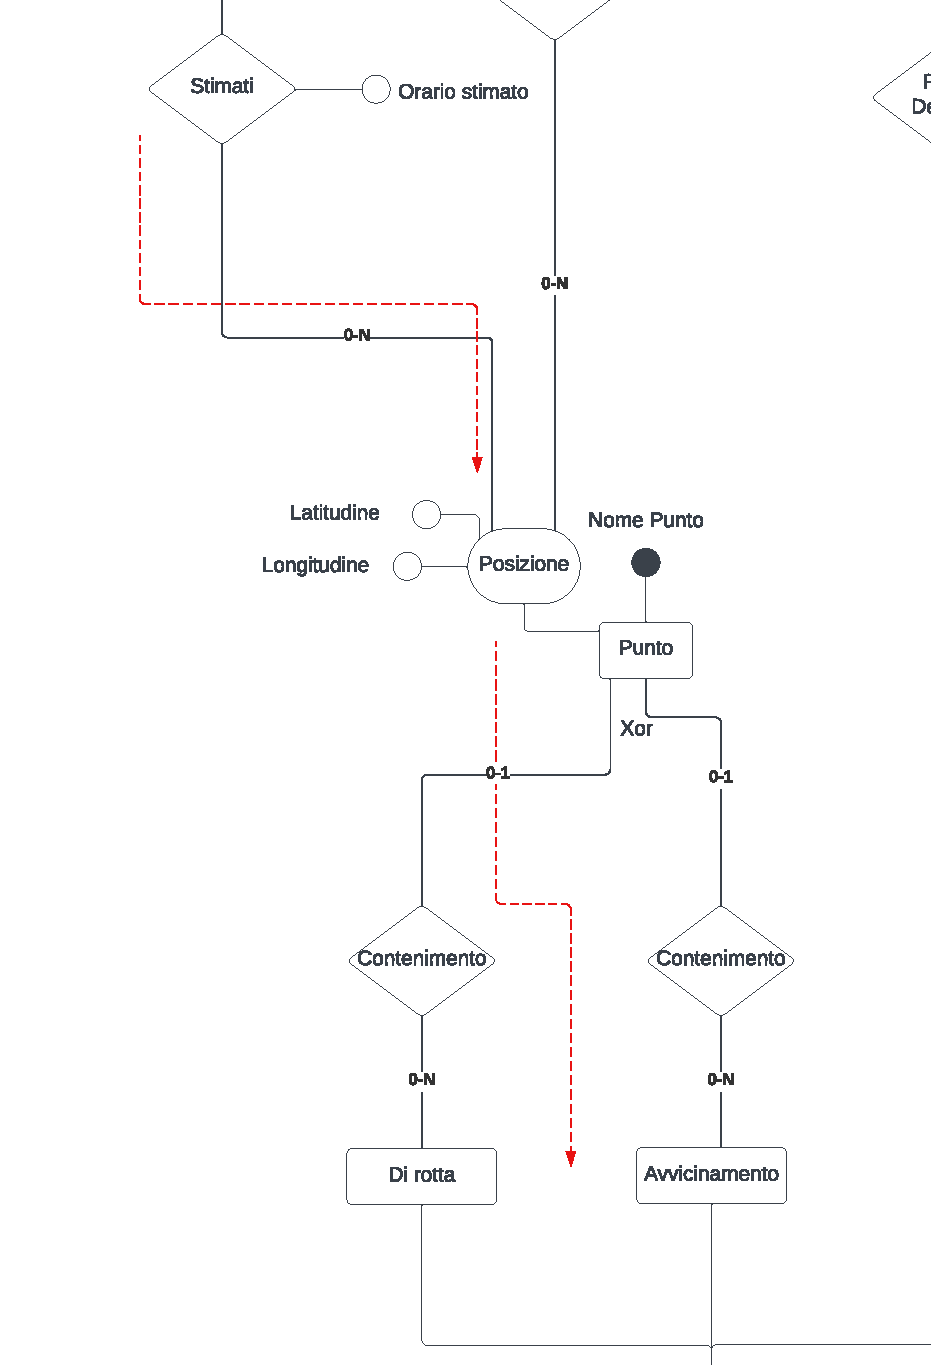
\includegraphics[width=10cm]{figures/BasicControllerarrowsp1.pdf}
      \caption{"Percorso per trovare l'occupazione"}
    \end{figure}
    
    \subsection*{OP11 - Aggiunta di una percorrenza}
    \begin{table}[H]
    \centering
    \rowcolors{2}{green!80!black!40}{white}
    \begin{tabular}{|c|c|c|c|}
    \hline
    \rowcolor{green!70!black!80}
    \textbf{Concetto} & \textbf{Costrutto} & \textbf{accessi} & \textbf{tipo}\\
    \hline
    Percorrenza & E & 1 & S \\\
    & & Totale: 1S, 0L, 1.000.000 al mese &\\
    \hline
    \end{tabular}
    \end{table}
  
\section{Raffinamento dello schema}
\section{Analisi delle ridondanze}
\section{Traduzione di entità e associazioni in relazioni}
\section{Schema relazionale finale}
\section{Traduzione delle operazioni in query SQL}